\documentclass{article}
\usepackage[margin = 2.54cm]{geometry} % set margin to traditional doc

%packages
\usepackage{graphicx} % Required for inserting images
\usepackage[most]{tcolorbox} %for creating environments
\usepackage{amsmath}
\usepackage{amssymb}
\usepackage{mathtools}
\usepackage{verbatim}
\usepackage[utf8]{inputenc}
\usepackage[dvipsnames]{xcolor} %for importing multiple colors
\usepackage{hyperref} %for creating links to different sections

\linespread{1.2} %controlling line spread

%define colors i like
\definecolor{myTeal}{RGB}{0,128,128}
\definecolor{myGreen}{RGB}{34,170,34}
\definecolor{mySapphire}{RGB}{15,82,186}
\definecolor{myEmerald}{RGB}{50.4, 130, 90}

%create math environments, can add [section] or [subsection] to add index counter based on sections/subsections
\newtheorem{define}{Definition}
\newtheorem{prop}{Proposition}
\newtheorem{thm}{Theorem}
\newtheorem{question}{Question}
\newtheorem{lemma}{Lemma}

%setup colored box environment for each math env above
\tcolorboxenvironment{define}{
    enhanced, colframe=myTeal!50!teal, colback=myTeal!10,
    arc=5mm, lower separated=false, fonttitle=\bfseries, breakable
}
\tcolorboxenvironment{prop}{
    enhanced, colframe=myGreen!50!black, colback=myGreen!15,
    arc=5mm, lower separated=false, fonttitle=\bfseries, breakable
}
\tcolorboxenvironment{thm}{
    enhanced, colframe=mySapphire!50!mySapphire, colback=mySapphire!15,
    arc=5mm, lower separated=false, fonttitle=\bfseries, breakable
}
\tcolorboxenvironment{question}{
    enhanced, colframe=blue!50!black, colback=blue!10,
    arc=5mm, lower separated=false, fonttitle=\bfseries, breakable
}
\tcolorboxenvironment{lemma}{
    enhanced, colframe=myEmerald!50!myEmerald, colback=myEmerald!10,
    arc=5mm, lower separated=false, fonttitle=\bfseries, breakable
}

%setup hyperlink within pdf
\hypersetup{
    colorlinks=true,
    linkcolor=blue,
    filecolor=magenta,      
    urlcolor=cyan,
    pdftitle={Overleaf Example},
    pdfpagemode=FullScreen,
}

%common command (add to template)
%general
\newcommand{\FF}{\mathbb{F}}
\newcommand{\NN}{\mathbb{N}}
\newcommand{\ZZ}{\mathbb{Z}}
\newcommand{\QQ}{\mathbb{Q}}
\newcommand{\RR}{\mathbb{R}}
\newcommand{\CC}{\mathbb{C}}

\newcommand{\Id}{\textmd{Id}} %identity
\newcommand{\lcm}{\textmd{lcm}}
\DeclarePairedDelimiter{\abs}{\lvert}{\rvert}
\DeclarePairedDelimiter{\norm}{\lVert}{\rVert}
\DeclarePairedDelimiter{\paran}{(}{)}%paranthesis
\DeclarePairedDelimiter{\bracket}{\langle}{\rangle}
\DeclarePairedDelimiter{\floor}{\lfloor}{\rfloor}

%algebra
\newcommand{\Gal}{\textmd{Gal}}
\newcommand{\Aut}{\textmd{Aut}}
\newcommand{\End}{\textmd{End}}
\newcommand{\Coker}{\textmd{Coker}}
\newcommand{\Hom}{\textmd{Hom}}
\newcommand{\Nil}{\textmd{Nil}}
\newcommand{\Char}{\textmd{char}}

%analysis
\newcommand{\Vol}{\textmd{Vol}}

%complex
\newcommand{\Real}{\textmd{Re}}
\newcommand{\Imag}{\textmd{Im}} %can also be used for Image
\newcommand{\Res}{\textmd{Res}}

%lie algebra
\newcommand{\gl}{\mathfrak{gl}}

%physics
\newcommand{\br}{\textbf{r}}
\newcommand{\bv}{\textbf{v}}
\newcommand{\ba}{\textbf{a}}

\title{Phys 103 HW2 Pass2}
\author{Zih-Yu Hsieh}

\begin{document}
\maketitle

\section*{Question 1}

\textbf{Pf:}
\subsection*{(a)}
In part (a), I misused the notation, where instead of $x(0)=A\cos(\phi)=0$, I should've written $0=x(0)=A\cos(\phi)$ (because we're given $x(0)=0$, not $A\cos(\phi)=0$).

\subsection*{(b)}
When doing the calculation, I forgot to assume that $t_0\in [0,\frac{2\pi}{w_1})$ is a local maximum of the function, but only assumed $x'(t_0)=0$ (which is not sufficient for local maximum). The rest of the calculation follows.

\hfil

\rule{15.6cm}{0.1mm}

\hfil

\section*{Question 3}

\textbf{Pf:}

\subsection*{(a)}
In this section when calculating the power dissipated by the damping force, I should've use that the power dissipated $P_\textmd{dissipated} = -F_\textmd{damp} v = bv^2$ instead (or else it's phrasing that the power dissipated is negative, or the damping force is providing positive power).

\hfil

\rule{15.6cm}{0.1mm}

\hfil

\section*{Question 4}

\textbf{Pf:}
\subsection*{(a)}
First, to explain more about the period, to prove the minimality of $T$, suppose for $t_1,t_2 \in [-\frac{T}{2},\frac{T}{2})$ it satisfies $f(t_1)=f(t_2)$, then since for index $i=1,2$, we have $-\frac{T}{2}\leq t_i < \frac{T}{2}$, hence $-\frac{1}{2}\leq \frac{t_i}{T}<\frac{1}{2}$, so $0\leq \frac{1}{2}+\frac{t_i}{T}<1$. Therefore, $\floor*{\frac{1}{2}+\frac{t_i}{T}}=0$. Hence, we get the following:
\begin{align}
    \frac{f_0t_1}{T}=f_0\paran*{\frac{t_1}{T}+\floor*{\frac{1}{2}+\frac{t_1}{T}}}=f(t_1)=f(t_2)=f_0\paran*{\frac{t_2}{T}+\floor*{\frac{1}{2}+\frac{t_2}{T}}}=\frac{f_0t_2}{T}
\end{align}
\begin{align}
    \implies t_1=t_2
\end{align}
(Note: above assumes $f_0, T\neq 0$).

This shows that the period can't be less than $T$ (or else there should be two distinct points in the above interval, where their function values are the same), which $T$ is the period.

\hfil

For the sketch, I think it's because the minus sign is too close, nevertheless I redrew the graph to make the minus sign more obvious:
\begin{figure}[h!]
    \begin{center}
        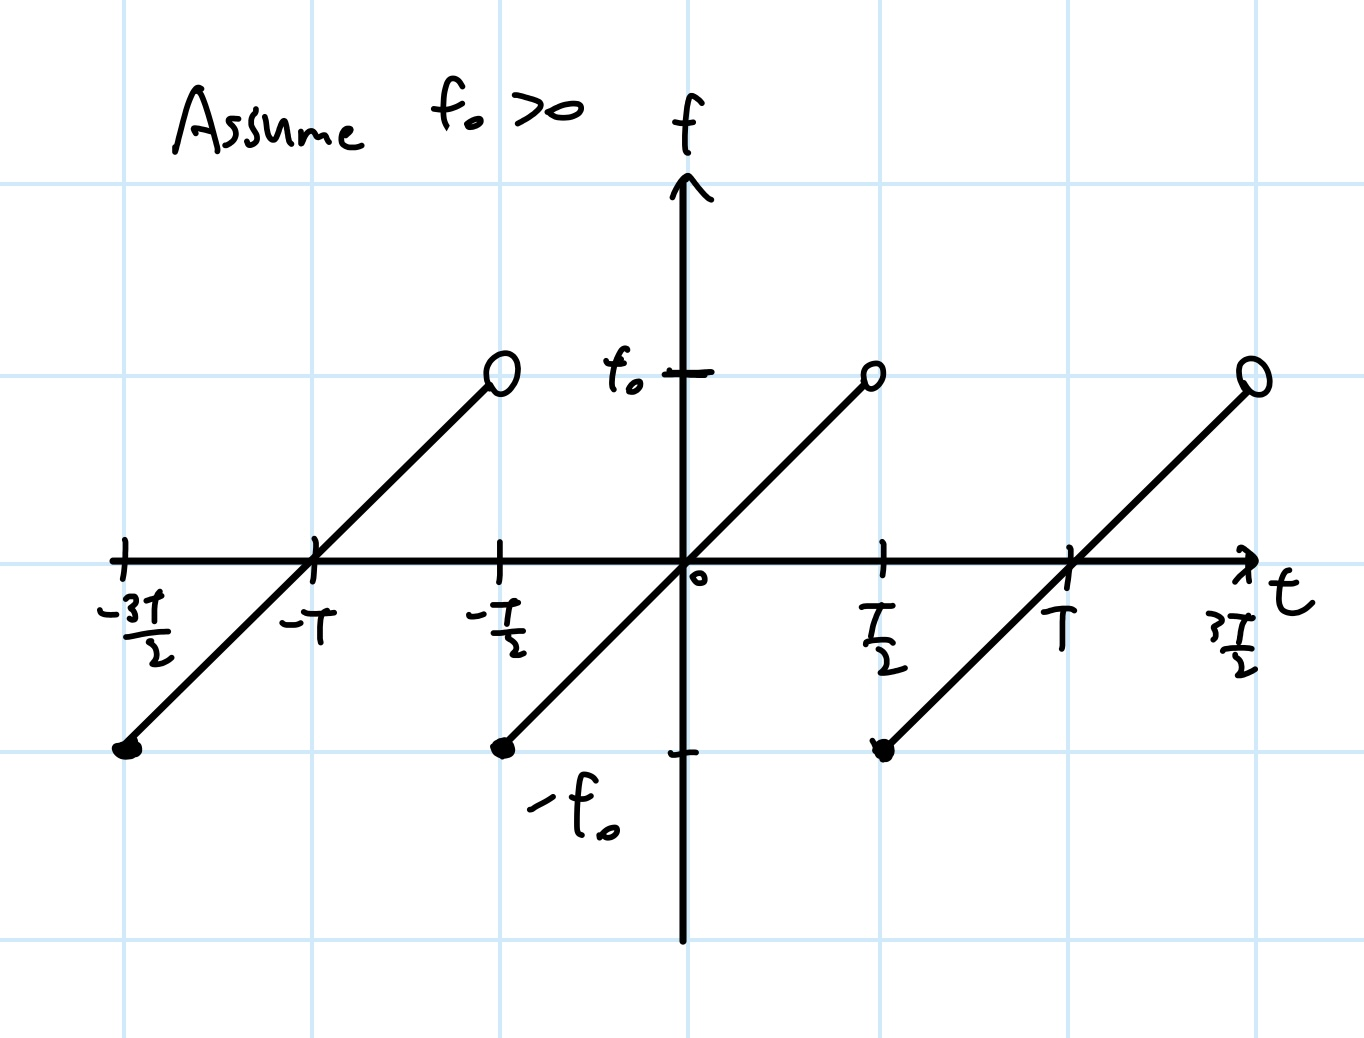
\includegraphics[width=70mm]{q4a.jpg}
    \end{center}
\end{figure}

\subsection*{(b)}
For the graph, I forgot to add the labels for each axis. Here's the modified version:
\begin{figure}[h!]
    \begin{center}
        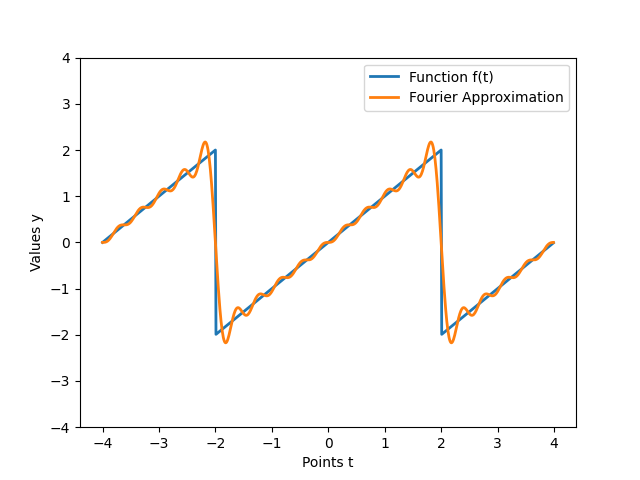
\includegraphics[width=70mm]{Figure_1.png}
    \end{center}
\end{figure}
Here's the modified code:
\rule{15.6cm}{0.1mm}
\begin{verbatim}
import matplotlib.pyplot as plt
import numpy as np
import math

#define constant (Note: both need to be positive)
T = 4
f_0 = 4

#define original function
def f(t):
   return f_0*(t/T - math.floor(1/2+t/T))

#define fourier series approximation, with n=10
def fourier(t):
   output = 0

   for n in range(1,11):
      output += (-1)**(n+1) * f_0 / (n* math.pi) * math.sin(2*n* math.pi * t/T)

   return output

#plot function
t = np.arange(-f_0, f_0, 0.01)

Function = []
Fourier = []
for i in range(len(t)):
   Function.append(f(t[i]))
   Fourier.append(fourier(t[i]))

plt.plot(t,Function, lw=2, label='Function f(t)')
plt.plot(t,Fourier, lw=2, label = 'Fourier Approximation')
plt.ylim(-T,T)
plt.xlabel("Points t")
plt.ylabel("Values y")

plt.legend()
plt.show()
\end{verbatim}
\rule{15.6cm}{0.1mm}

\break

\section*{Question 6}

\textbf{Pf:}
\subsection*{(a)}
I forgot to answer the question whether it's going faster or slower eventually. This depends on the context:
\begin{itemize}
    \item If the oscillator is undamped, then the amplitude of the system is always the same. Hence, the period of the system stays constant, which it's not slower or faster.
    \item If the oscillator is damped, then its maximum amplitude is constantly decreasing, so when maximum amplitude is lower, with $T=\frac{2\pi}{w_0}\paran*{1+\frac{\phi_{\max}^2}{16}}$, we get that $T$ is decreasing. Hence, each cycle actually takes time less than $2$ seconds; Since each cycle takes less time, within the same time elapsed there are more cycles happened than default, hence it records a higher time elapsed than the actual time, showing that the pendulum eventually runs faster.
\end{itemize}
\subsection*{(b)}
For this question I should include the units for time, so I should say $2$ seconds instead (and say $86400$ seconds in the integrand).

\end{document}